\documentclass[11pt]{article}
\usepackage[T1]{fontenc}
\usepackage{lmodern}
\usepackage[letterpaper,margin=1.02in]{geometry}
\usepackage{amsmath,amssymb,amsthm,booktabs,array,microtype,tikz}
\usepackage{xurl}
\usepackage[colorlinks=true,allcolors=bluegreen]{hyperref}
\definecolor{bluegreen}{RGB}{22,83,91}
\hypersetup{pdftitle={Polynomial images of Stoneham numbers with an odd prime-power parameter},pdfauthor={}}
\newtheorem{theorem}{Theorem}
\newtheorem{lemma}[theorem]{Lemma}
\newtheorem{corollary}[theorem]{Corollary}
\newtheorem{proposition}[theorem]{Proposition}
\newcommand{\R}{\mathbb R}
\newcommand{\Q}{\mathbb Q}
\newcommand{\Z}{\mathbb Z}
\newcommand{\N}{\mathbb N_0}
\newcommand{\T}{\mathbb T}
\newcommand{\ee}[1]{\exp(2\pi i #1)}
\DeclareMathOperator{\den}{den}
\newcommand{\baseurl}{https://github.com/eldernos/MathematicsResearch/blob/a09e011720bc74396a27f4cb3ce2d8a5b3ce5035}
\newcommand{\addurl}{https://github.com/eldernos/MathematicsResearch/blob/afc35498a377fce8ce1d216e820990e54c7ba32c}
\newcommand{\kernel}[3]{\href{\baseurl/NormalityChecker/#1.lean\#L#2}{#3}}
\newcommand{\added}[3]{\href{\addurl/NormalityChecker/#1.lean\#L#2}{#3}}
\setlength{\emergencystretch}{1.5em}
\raggedbottom

\begin{document}
\begin{center}
{\LARGE\bfseries Polynomial images of Stoneham numbers\\with an odd prime-power parameter\par}
\vspace{0.6em}
{\small Research manuscript \enspace $\cdot$ \enspace 24 November 2026}
\end{center}
\begin{abstract}
Let $b\ge2$ be an integer, $p$ an odd prime with $p\nmid b$, and $c$ a positive power of $p$.
For the standard Stoneham constant $\alpha_{b,c}=\sum_{j\ge1}c^{-j}b^{-c^j}$,
every nonconstant rational polynomial $P(\alpha_{b,c})$ is normal in base $b$.
More generally, a rational combination of products of $\alpha_{b^m,p^e}$ is normal
if it has one monomial of strictly greatest degree with nonzero coefficient.
The proof identifies a nonvanishing inclusion--exclusion numerator for each upper set
of reflected exponents. Compactness bounds the loss in the reduced prefix denominator
uniformly across all insertion patterns.
Distinct positive powers of one generator have jointly uniformly distributed radix orbits.
For the square of $\alpha_{2,3}$ we give the exact prefix denominators.
The binary discrepancy of $\alpha_{2,3}\alpha_{2,5}$ has upper limit at most $43/45$.
Ridout's theorem gives transcendence both for this product and for the one-axis combinations above.
\end{abstract}

\section{Normality in the defining radix}

For integers $b,c\ge2$ put
\begin{equation}\label{eq:stoneham}
 \alpha_{b,c}=\sum_{j=1}^{\infty}\frac{1}{c^j b^{c^j}} .
\end{equation}
Put $\T=\R/\Z$. For $x\in\R$, write $T_b^n x=\{b^nx\}$, with fractional part in $[0,1)$.
The real number $x$ is \emph{normal in base $b$} if for every $k\ge1$ and $0\le h<b^k$
the proportion of $0\le n<N$ for which $T_b^n x\in[h/b^k,(h+1)/b^k)$ tends to $b^{-k}$.
Digit words are counted with overlaps and leading zeros, using the terminating convention for radix rationals.
Approximating an arbitrary interval by unions of these intervals shows that normality
is equivalent to uniform distribution of $(T_b^n x)_{n\ge0}$ in $[0,1)$.

\begin{theorem}[Polynomial images]\label{thm:main}
Let $b\ge2$, let $p$ be an odd prime coprime to $b$, and let $e\ge1$ be an integer.
For every nonconstant polynomial $P\in\Q[X]$, the number $P(\alpha_{b,p^e})$ is normal in base $b$.
\end{theorem}

In particular, every positive power of $\alpha_{2,3}$ is binary normal.
For products we count degree with multiplicity. Choose positive integers $m_i,e_i$
independently in each factor and put
\begin{equation}\label{eq:monomial}
 M=\prod_{i=1}^d \alpha_{b^{m_i},p^{e_i}},\qquad \deg M=d.
\end{equation}
For $d=0$ we use the empty product $M=1$.

\begin{theorem}[One monomial of highest degree]\label{thm:monomial}
Fix $b,p$ as in Theorem~\ref{thm:main}. Let $s\ge0$ and let $M,M_1,\ldots,M_s$
be monomials of the form \eqref{eq:monomial} for these $b,p$, with $\deg M=d\ge1$
and $\deg M_\nu<d$ for $1\le\nu\le s$. Take $A,A_1,\ldots,A_s\in\Q$ with $A\ne0$.
Then $AM+\sum_{\nu=1}^s A_\nu M_\nu$ is normal in base $b$.
In particular, every nonempty product \eqref{eq:monomial} is normal in that base.
\end{theorem}

The choices $m_1=m_2=1$, $e_1=1$, $e_2=2$ give the binary-normal number
$\alpha_{2,3}\alpha_{2,9}$. The strict degree inequality prevents the lower-degree terms from canceling the leading
$p$-power in the reduced denominator. In a general multivariate
polynomial several terms of maximal degree can contribute at the same denominator order.

\subsection*{Relation to earlier results}
Stoneham established normality for specific constants including $\alpha_{2,3}$ by studying
digits in periodic fractions \cite{stoneham}. Kano reports A.~N.~Korobov's criterion for
$\sum a^{-\lambda_j}b^{-\mu_j}$ with increasing exponents and $\mu_j\ge a^{\lambda_j}$
includes the individual standard generator by taking $\lambda_j=j$ and $\mu_j=a^j$
\cite[pp.~909--910]{kano}; see also \cite{korobov}. Bailey and Crandall give the coprime-parameter theorem for
\eqref{eq:stoneham} and a more general lacunary-series criterion
\cite[Theorem 4.8 and Corollary 4.9]{bc}. Thus degree one in Theorem~\ref{thm:main}
also follows by Wall's rational affine invariance theorem \cite{wall}.

Wagner constructed explicit rings of normal numbers \cite{wagner}.
Kano and Shiokawa proved normality for polynomial combinations of lacunary
generators under their separation conditions \cite[Theorems 4--5]{ks}.
For an individual generator in \eqref{eq:stoneham}, taking $a=c$ gives
$\lambda_j/\mu_{j-1}=j/c^{j-1}\to0$ and $(\log\mu_j)/\lambda_j=\log c$.
Both quantities must diverge in conditions (15)--(16) of their construction.
Kano's comparison gives the corresponding growth requirements in Wagner's construction
\cite[pp.~909--911]{kano}. The older results establish polynomial normality for
explicit families. N.~M.~Korobov studied simultaneous normality under the name of conjunctly
normal numbers \cite{jointkorobov}. Corollary~\ref{cor:joint} takes the coordinates to be
distinct powers of the same classical generator.

Vandehey's fixed-prime-support estimate supplies the analytic implication from reduced
denominators to uniformity \cite[Corollary 1.2 in the preprint]{vandehey}. Theorem 7.4 of that version treats a series
with unit numerators, strictly increasing coefficient denominators in a divisibility chain,
and a gap condition. Even in a square, two ordered pairs may contribute at one location,
and their combined coefficients can cancel a denominator layer.
Bailey and Borwein asked about the normality of sums of two standard Stoneham constants \cite[\S4]{bb}.
The 2026 repository preprint \cite{twosum} proves normality of
$\alpha_{b,c}+\alpha_{b,d}$ whenever $\gcd(b,cd)=1$, also for independent parameters.
Its two linear terms have equal degree. The mixed product studied in
Section~\ref{sec:mixed} requires estimates at the locations $3^i+5^j$.
Theorem~\ref{thm:main} treats nonlinear images of the particular generators
\eqref{eq:stoneham} on an odd prime-power axis. For these generators the inclusion--exclusion numerator bounds the loss of
$p$-powers uniformly when distinct tuples enter the same prefix. The example after
Lemma~\ref{lem:numerator} explains why this argument requires an odd prime.

\section{The numerator of an upper set}

Fix $d\ge1$ and positive integer weights $e=(e_1,\ldots,e_d)$. For
$v\in\N^d$ write $|v|_e=\sum_i e_i v_i$. Use the coordinatewise order on $\N^d$.
For an upper set $U$, let
\[
 H_U(z)=\sum_{v\in U}z^{|v|_e}\ \in\Z[[z]].
\]
Each coefficient is a finite sum. At $z=p$ the same series converges in $\Z_p$,
since only finitely many terms have valuation below any prescribed integer.

\begin{lemma}[Orthant numerator]\label{lem:numerator}
Every nonempty upper set $U\subset\N^d$ has a polynomial $K_U\in\Z[z]$ such that
\[
 H_U(z)=\frac{K_U(z)}{\prod_{i=1}^d(1-z^{e_i})},\qquad K_U(1)=1.
\]
Consequently $K_U(p)\equiv1\pmod{p-1}$ and $H_U(p)\ne0$ for every odd prime $p$.
\end{lemma}
\begin{proof}
Dickson's lemma gives finitely many minimal vectors $v_1,\ldots,v_s$ in $U$.
Indeed, every infinite sequence in $\N$ has an infinite nondecreasing subsequence.
Applying this successively in each of $d$ coordinates rules out an infinite antichain.
Every vector of $U$ lies above a minimal vector by descent in total degree.
Hence $U$ is the union of the orthants $v_j+\N^d$.
For $\varnothing\ne J\subseteq\{1,\ldots,s\}$ let $v_J$ be the coordinatewise maximum
of the $v_j$ with $j\in J$. Their orthants intersect in $v_J+\N^d$, with generating
function $z^{|v_J|_e}/\prod_i(1-z^{e_i})$. Inclusion--exclusion yields
\begin{equation}\label{eq:K}
 K_U(z)=\sum_{\varnothing\ne J\subseteq\{1,\ldots,s\}}
             (-1)^{|J|+1}z^{|v_J|_e}.
\end{equation}
Evaluating the numerator at $1$ gives $\sum_{r=1}^{s}(-1)^{r+1}\binom{s}{r}=1$, where $s$ is the number of minimal vectors. Since $p\equiv1\bmod(p-1)$,
the ordinary integer $K_U(p)$ is nonzero when $p-1>1$. The geometric denominator
is a $p$-adic unit. This proves the assertion even when $p$ divides $K_U(p)$.
\end{proof}

The odd-prime hypothesis enters at this point. For $d=2$ and
$U=\N^2\setminus\{(0,0)\}$ with both weights one, $K_U(z)=2z-z^2$.
Thus the leading numerator can vanish at $p=2$.

\begin{lemma}[Uniform precision]\label{lem:compact}
Fix an odd prime $p$, weights $e$, and $v_*\in\N^d$.
There is an $L\ge1$ such that $H_U(p)\not\equiv0\bmod p^L$
for every upper set $U$ containing $v_*$.
\end{lemma}
\begin{proof}
If the assertion fails, choose $U_\ell$ containing $v_*$ with $p^\ell\mid H_{U_\ell}(p)$
for every $\ell\ge1$. By a diagonal extraction over the countable set $\N^d$,
the indicators converge pointwise on a subsequence, eventually constant at each vector.
Their limit is the indicator of an upper set $U$ containing $v_*$. At a fixed precision $r$,
only $|v|_e<r$ can contribute. Membership of all these vectors eventually agrees with $U$.
Thus $H_U(p)\equiv0\bmod p^r$ for every $r$, contrary to Lemma~\ref{lem:numerator}.
\end{proof}

For example, take $d=2$, $e_1=e_2=1$, $p=3$, and
$U=\{(i,j):3^{-i}+3^{-j}\le10/9\}$. Its minimal vectors are $(0,2),(1,1),(2,0)$.
The joins of $(0,2)$ and $(2,0)$ and of all three vectors coincide. Formula~\eqref{eq:K}
reduces to $K_U(z)=3z^2-2z^3$, so $K_U(3)=-27$.
Here $v_3(H_U(3))=3$.

\begin{figure}[ht]
\centering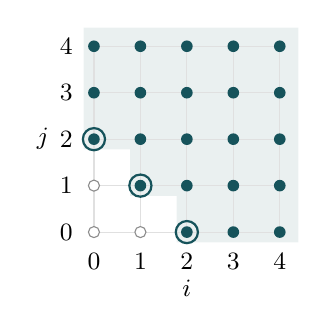
\begin{tikzpicture}[x=.59cm,y=.59cm,font=\small]
\fill[bluegreen!9] (-.22,1.78) -- (.78,1.78) -- (.78,.78) -- (1.78,.78) -- (1.78,-.22) -- (4.4,-.22) -- (4.4,4.4) -- (-.22,4.4) -- cycle;
\draw[step=1,black!12] (0,0) grid (4,4);
\draw[black!45,fill=white] (0,0) circle (2pt);
\draw[black!45,fill=white] (0,1) circle (2pt);
\fill[bluegreen] (0,2) circle (2.1pt);
\fill[bluegreen] (0,3) circle (2.1pt);
\fill[bluegreen] (0,4) circle (2.1pt);
\draw[black!45,fill=white] (1,0) circle (2pt);
\fill[bluegreen] (1,1) circle (2.1pt);
\fill[bluegreen] (1,2) circle (2.1pt);
\fill[bluegreen] (1,3) circle (2.1pt);
\fill[bluegreen] (1,4) circle (2.1pt);
\fill[bluegreen] (2,0) circle (2.1pt);
\fill[bluegreen] (2,1) circle (2.1pt);
\fill[bluegreen] (2,2) circle (2.1pt);
\fill[bluegreen] (2,3) circle (2.1pt);
\fill[bluegreen] (2,4) circle (2.1pt);
\fill[bluegreen] (3,0) circle (2.1pt);
\fill[bluegreen] (3,1) circle (2.1pt);
\fill[bluegreen] (3,2) circle (2.1pt);
\fill[bluegreen] (3,3) circle (2.1pt);
\fill[bluegreen] (3,4) circle (2.1pt);
\fill[bluegreen] (4,0) circle (2.1pt);
\fill[bluegreen] (4,1) circle (2.1pt);
\fill[bluegreen] (4,2) circle (2.1pt);
\fill[bluegreen] (4,3) circle (2.1pt);
\fill[bluegreen] (4,4) circle (2.1pt);
\draw[bluegreen,thick] (0,2) circle (4pt);
\draw[bluegreen,thick] (1,1) circle (4pt);
\draw[bluegreen,thick] (2,0) circle (4pt);
\foreach \i in {0,...,4} {\node[below] at (\i,-.25) {\i}; \node[left] at (-.25,\i) {\i};}
\node at (2,-1.2) {$i$}; \node at (-1.1,2) {$j$};
\end{tikzpicture}

\caption{Reflected insertion lattice at the cut $10/9$.
Solid points satisfy $3^{-i}+3^{-j}\le10/9$. Circles around solid points mark the three minimal vectors.}
\label{fig:lattice}
\end{figure}

\section{Rational prefixes on one prime axis}

For a monomial $M$ as in \eqref{eq:monomial} and
$j=(j_1,\ldots,j_d)\in\Z_{\ge1}^d$, put
\[
 s(j)=\sum_i m_i p^{e_i j_i},\qquad w(j)=\sum_i e_i j_i,\qquad
 R_n(M)=\sum_{s(j)\le n}p^{-w(j)} b^{n-s(j)} .
\]
Each ordered tuple is retained, including all tuples having the same location.
The degree-zero convention is $R_n(1)=b^n$.
For a rational number $r$ write $\den(r)$ for its positive reduced denominator.

\begin{lemma}[Real tail and denominator]\label{lem:den}
For every fixed monomial $M$ of degree $d\ge0$, $b^nM-R_n(M)\to0$.
For all $n\ge1$, with $k=\lfloor\log_p n\rfloor$, one has $\den(R_n(M))\mid p^{dk}$.
If $d\ge1$, there are integers $C\ge0$ and $k_0\ge1$ with $dk_0\ge C$ such that
$p^{dk-C}\mid\den(R_n(M))$ for every $k\ge k_0$.
\end{lemma}
\begin{proof}
Multiplication of absolutely convergent series gives
$M=\sum_j p^{-w(j)}b^{-s(j)}$. The contribution of each fixed tuple to the shifted
tail eventually vanishes. Its absolute value is bounded by $p^{-w(j)}$, whose sum
over tuples is $\prod_i(p^{e_i}-1)^{-1}$. Dominated convergence gives the first assertion.

At degree zero the denominator is one. In positive degree, $s(j)\le n$ implies
$e_i j_i\le k$ for all $i$, proving the upper divisibility at every cutoff. Write
$h_i=\lfloor k/e_i\rfloor$, $r_i=k-e_i h_i$, $A=\sum_i e_i h_i$.
Thus $dk-\sum_i(e_i-1)\le A\le dk$ and $p^A R_n(M)$ is integral.
Reflect by $v_i=h_i-j_i$. With $t=n/p^k\in[1,p)$ the insertion condition becomes
\[
 U=\Big\{v\in\N^d:\ \sum_i m_i p^{-r_i-e_i v_i}\le t\Big\}.
\]
The actual reflected tuples must also satisfy $v_i<h_i$. This upper set contains
$(J,\ldots,J)$ whenever $J$ is large enough that $p^J\ge\sum_i m_i$, independently
of $k,n$. Choose $L$ from Lemma~\ref{lem:compact} for this anchor. Modulo $p^L$ only
$|v|_e<L$ matters. Uniformly for these finitely many $v$, large $k$ ensures
$v_i<h_i$ and $e_i(h_i-v_i)\ge L$ in every coordinate. Thus every tuple contributing modulo $p^L$ has positive original indices.

The powers $(b^{-1})^{p^s}$ in $(\Z/p^L\Z)^\times$ have one common value $u_L$
for $s\ge L$. Indeed $\varphi(p^L)=p^{L-1}(p-1)$ divides
$p^{s+1}-p^s$. On all contributing tuples $b^{-s(j)}$ consequently has the
common value $u_L^{\sum_i m_i}$. Since $A-w(j)=|v|_e$, this gives
\begin{equation}\label{eq:frozen}
 p^A b^{-n}R_n(M)\equiv u_L^{\sum_i m_i} H_U(p)\pmod {p^L}.
\end{equation}
The congruence is in $\Z_p$, where $b$ is invertible. Its right side is nonzero
modulo $p^L$. Thus $v_p(p^A R_n(M))<L$. Reduction loses at most $L-1$ powers
from the denominator $p^A$, as required.
\end{proof}

\section{From denominator survival to digit frequencies}

Fix a finite set $S$ of primes coprime to $b$ and a real $D>0$.
For each $\varepsilon>0$ the short-orbit estimate gives $q_0$ such that for every
integer $B\ge1$ and reduced $a/q$ with $q_0\le q\le B^D$ supported on $S$,
the mean below has absolute value at most $\varepsilon$. Equivalently,
\begin{equation}\label{eq:short}
 \frac1B\sum_{i=0}^{B-1}\ee{a b^i/q}\longrightarrow0
 \quad\text{as }q\longrightarrow\infty .
\end{equation}
This follows from Vandehey \cite[Corollary 1.2 in the preprint]{vandehey} with $B\ge q^{1/D}$.
Changing the starting power amounts to multiplying $a$ by a unit modulo $q$.
Differencing at multiples of the orders of $b$ modulo divisors of $q$ gives the
qualitative bound used in the formal proof (Table~\ref{tab:formal}). For a fixed nonzero Fourier frequency $h$,
reducing $ha/q$ loses at most a factor $|h|$, so \eqref{eq:short} applies to that frequency too.

\begin{proof}[Proof of Theorems~\ref{thm:monomial} and~\ref{thm:main}]
First suppose the coefficients are integers and denote their combination by $x$.
Use the same combination of the $R_n$ to define $R_n(x)$. Every term of lower degree
has denominator dividing $p^{(d-1)k}$. By Lemma~\ref{lem:den}, the leading term,
after multiplication by its nonzero coefficient $A$, has denominator divisible by
$p^{dk-C-v_p(A)}$. For $k>C+v_p(A)$ its pole is strictly larger than every lower pole.
The ultrametric inequality with unequal valuations shows that its pole order persists
in the sum. Consequently $q_n=\den(R_n(x))$ tends uniformly to infinity at late
positions and divides $p^{dk}\le n^d$. Also $b^nx-R_n(x)\to0$.

Fix a nonzero integer frequency $h$. To estimate its mean up to $N$, discard
positions below $\lfloor\sqrt N\rfloor$, then partition the rest into blocks of length
$B=\lfloor\sqrt N\rfloor$, discarding the final incomplete block.
There are $O((1+\log N)^d)$ insertion tuples up to $N$ in the fixed list of monomials.
Discard blocks containing an insertion. All discarded positions together number
$O(B(1+\log N)^d)=o(N)$. In a retained block starting at $n$,
$R_{n+i}(x)=b^iR_n(x)$ for $0\le i<B$.
Its starting denominator tends uniformly to infinity and $q_n\le N^d\le B^{3d}$
for large $N$. Equation~\eqref{eq:short} gives a uniformly vanishing block mean
for $\ee{h R_{n+i}(x)}$. The real tail and
$|\ee{u}-\ee{v}|\le2\pi |u-v|$ transfer this bound to $\ee{h b^{n+i}x}$.
Summing the block bounds and using the trivial bound one on discarded positions proves
$\frac1N\sum_{n<N}\ee{h b^nx}\to0$. Weyl's criterion \cite{weyl} gives normality.

For rational coefficients choose $D\ge1$ clearing all denominators. Normality
of $Dx$ implies normality of $x$. Indeed, every subsequential weak limit
$\mu$ of the empirical measures of $T_b^nx$ on $\T$ is invariant under multiplication
by $b$ by telescoping. Its image under multiplication by $D$ is Lebesgue measure.
A Lebesgue-null set has null image under this finite covering (cover it by intervals
of arbitrarily small total length), so $\mu$ is absolutely continuous. Its Fourier
coefficients satisfy $\widehat\mu(h)=\widehat\mu(b^k h)$ and tend to zero at infinity
by the Riemann--Lebesgue lemma. Hence $\mu$ is Lebesgue measure. Compactness gives
convergence of the entire sequence. This proves Theorem~\ref{thm:monomial}.
Taking all $m_i=1$ and all $e_i=e$ in each degree proves Theorem~\ref{thm:main}.
\end{proof}

\begin{corollary}[Simultaneous powers]\label{cor:joint}
Write $\alpha=\alpha_{b,p^e}$ under the hypotheses of Theorem~\ref{thm:main}.
For distinct positive integers $r_1,\ldots,r_d$ and $0\le a_i\le c_i\le1$,
\[
 \lim_{N\to\infty}\frac1N\#\{0\le n<N:\ a_i\le\{b^n\alpha^{r_i}\}<c_i
                    \ \text{for every } i\}
       =\prod_{i=1}^d(c_i-a_i).
\]
\end{corollary}
\begin{proof}
For a nonzero $h\in\Z^d$ the polynomial $\sum_i h_i X^{r_i}$ is nonconstant:
any nonzero $h_j$ is the coefficient of its own positive degree $r_j$. Theorem~\ref{thm:main}
therefore makes the mean of the torus character at $h$ tend to zero by the
one-dimensional Weyl criterion. The character at zero averages to one.
The character span is uniformly dense in $C(\T^d)$ by Stone--Weierstrass, so
every continuous test function has limiting average equal to its Haar integral.
For an interval of length $\ell$, continuous periodic functions with values in $[0,1]$
can bound its indicator from below and above with integrals between
$\max(0,\ell-2\delta)$ and $\min(1,\ell+2\delta)$: taper linearly across collars of
width $\delta$ at both endpoints, inside for the lower bound and outside for the upper.
Use the constant lower function $0$ if $\ell\le2\delta$, and the constant upper
function $1$ if $\ell+2\delta\ge1$.
Multiplying the bounds over all coordinates gives continuous bounds for the box.
Their integrals factor, and letting $\delta\downarrow0$ proves the formula.
The empty product gives the same formula in dimension zero.
\end{proof}

\begin{table}[ht]
\centering\begin{tabular}{c@{\qquad}rrrr}\toprule
&\multicolumn{4}{c}{Word in $\alpha^2$}\\
Word in $\alpha$ & 00 & 01 & 10 & 11 \\ \midrule
00 & 239 & 276 & 263 & 264 \\
01 & 250 & 245 & 271 & 252 \\
10 & 255 & 253 & 253 & 257 \\
11 & 268 & 255 & 242 & 253 \\
\bottomrule\end{tabular}

\caption{Exact counts of simultaneous two-bit words for $\alpha_{2,3}$ and
$\alpha_{2,3}^2$ at the first 4096 starting positions.
The limiting proportion in each cell is $1/16$ by Corollary~\ref{cor:joint}.}
\end{table}

\section{Exact denominators for the binary square}

Write $\alpha=\alpha_{2,3}$ and let
\[
 R_n=\sum_{\substack{i,j\ge1\\3^i+3^j\le n}}
              \frac{2^{n-3^i-3^j}}{3^{i+j}},\qquad q_n=\den(R_n).
\]
The first insertion is at $6$. These are shifted prefixes of the \emph{square}:
truncating the generator and then squaring it would select a different set of ordered pairs.

\begin{theorem}[Square profile]\label{thm:square}
For $k\ge4$ and $3^k\le n<3^{k+1}$, the denominator is $q_n=3^v$ with
\[
\begin{array}{c|c}
 \text{interval for }n & v\\ \hline
 {}[3^k,3^k+3^{k-2})&2k-2\\
 {}[3^k+3^{k-2},3^k+3^{k-1})&2k-3\\
 {}[3^k+3^{k-1},2\cdot3^k)&2k-1\\
 {}[2\cdot3^k,3^{k+1})&2k .
\end{array}
\]
For $0\le n<81$ the complete list is
\[
\begin{array}{c|rrrrrrr}
 n &[0,6)&[6,12)&[12,18)&[18,30)&[30,36)&[36,54)&[54,81)\\ \hline
 q_n&1&9&27&81&9&243&729 .
\end{array}
\]
In particular $n^2<243q_n$ and $q_n\le n^2$ for $n\ge81$.
\end{theorem}
\begin{proof}
All pairs with $i,j\le k-1$ occur by $3^k$, and all further pairs on this shell
have an index $k$. The distinct pairs $(k,j),(j,k)$ arrive at $3^k+3^j$ for $j<k$.
For the largest degree $D=i+j$ present, the residue of $3^D R_n$ modulo $3$ is
$2^n$ times the number of pairs of degree $D$. Modulo $9$, it is $2^n$ times
that number plus $2^n\cdot3$ times the number of pairs of degree $D-1$:
each location $3^i+3^j$ is divisible by $6$ and $2^6\equiv1\bmod9$.

On the first interval the only maximal pair is $(k-1,k-1)$. On the second,
two additional pairs of degree $2k-2$ have arrived, namely $(k,k-2)$ and its transpose.
There are four pairs of degree $2k-3$, namely $(k-1,k-2),(k,k-3)$ and their transposes.
After removing $2^n$ the residue is $3+3\cdot4\equiv6\bmod9$; precisely one factor
of three cancels. On the third interval the top layer consists of $(k,k-1)$ and
its transpose, and on the fourth it consists of $(k,k)$. Both counts give units
modulo three.

Before $81$ the only locations are $6,12,18,30,36,54$, with jumps in the shifted prefix
$1/9,2/27,1/81,2/81,2/243,1/729$, respectively. Starting with $R_0=0$, double
the previous prefix at each step and add the indicated jump at its location.
In particular $R_{30}=16952434/9$, $R_{35}=542477888/9$, and
$R_{36}=29293805954/243$. Between jumps doubling preserves the denominator.
At $k=3$ both $(3,0)$ and $(0,3)$ are absent because $i,j\ge1$.
The last assertions follow from $3^{2k-3}\le q_n\le3^{2k}$ and
$3^k\le n<3^{k+1}$.
\end{proof}

\begin{figure}[ht]
\centering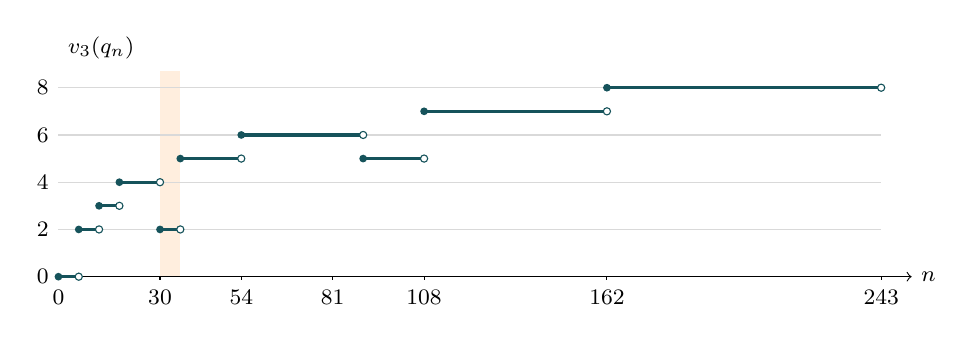
\begin{tikzpicture}[x=.043cm,y=.30cm,font=\footnotesize]
\fill[orange!13] (30,0) rectangle (36,8.7);
\foreach \i in {0,2,4,6,8} {\draw[black!15] (0,\i) -- (243,\i); \node[left] at (0,\i) {\i};}
\foreach \i in {0,30,54,81,108,162,243} {\draw (\i,-.14) -- (\i,0); \node[below] at (\i,-.14) {\i};}
\draw[->] (0,0) -- (252,0) node[right] {$n$};
\node[anchor=south west] at (0,8.8) {$v_3(q_n)$};
\draw[bluegreen,very thick] (0,0) -- (6,0);
\fill[bluegreen] (0,0) circle (1.4pt);
\draw[bluegreen,fill=white] (6,0) circle (1.3pt);
\draw[bluegreen,very thick] (6,2) -- (12,2);
\fill[bluegreen] (6,2) circle (1.4pt);
\draw[bluegreen,fill=white] (12,2) circle (1.3pt);
\draw[bluegreen,very thick] (12,3) -- (18,3);
\fill[bluegreen] (12,3) circle (1.4pt);
\draw[bluegreen,fill=white] (18,3) circle (1.3pt);
\draw[bluegreen,very thick] (18,4) -- (30,4);
\fill[bluegreen] (18,4) circle (1.4pt);
\draw[bluegreen,fill=white] (30,4) circle (1.3pt);
\draw[bluegreen,very thick] (30,2) -- (36,2);
\fill[bluegreen] (30,2) circle (1.4pt);
\draw[bluegreen,fill=white] (36,2) circle (1.3pt);
\draw[bluegreen,very thick] (36,5) -- (54,5);
\fill[bluegreen] (36,5) circle (1.4pt);
\draw[bluegreen,fill=white] (54,5) circle (1.3pt);
\draw[bluegreen,very thick] (54,6) -- (90,6);
\fill[bluegreen] (54,6) circle (1.4pt);
\draw[bluegreen,fill=white] (90,6) circle (1.3pt);
\draw[bluegreen,very thick] (90,5) -- (108,5);
\fill[bluegreen] (90,5) circle (1.4pt);
\draw[bluegreen,fill=white] (108,5) circle (1.3pt);
\draw[bluegreen,very thick] (108,7) -- (162,7);
\fill[bluegreen] (108,7) circle (1.4pt);
\draw[bluegreen,fill=white] (162,7) circle (1.3pt);
\draw[bluegreen,very thick] (162,8) -- (243,8);
\fill[bluegreen] (162,8) circle (1.4pt);
\draw[bluegreen,fill=white] (243,8) circle (1.3pt);
\end{tikzpicture}

\caption{Exact finite computation of the square denominator through $n=242$.
The shaded interval is $[30,36)$. The plotted heights come from the rational
recurrence in the proof of Theorem~\ref{thm:square}.}
\end{figure}

\section{A product on two prime axes}\label{sec:mixed}

For an interval $I=[a,c)\subset[0,1)$ let $F_N(I;x,b)$ denote its empirical frequency
among $T_b^n x$, $0\le n<N$. We use the extreme interval discrepancy
\[
 D_\infty^{(b)}(x)=\limsup_{N\to\infty}\sup_{0\le a<c\le1}
          |F_N([a,c);x,b)-(c-a)|.
\]
Write $D_\infty=D_\infty^{(2)}$.

\begin{theorem}[Two independent primes]\label{thm:mixed}
The product $x=\alpha_{2,3}\alpha_{2,5}$ is irrational and $D_\infty(x)\le43/45$.
\end{theorem}
\begin{proof}
Its ordered terms have location $3^i+5^j$ and coefficient $1/(3^i5^j)$ for $i,j\ge1$.
Define $R_n$ by retaining all terms with location at most $n$ and multiplying by $2^n$.
The summable product of the two geometric coefficient sequences gives $2^nx-R_n\to0$
as in Lemma~\ref{lem:den}. The denominator of $R_n$ divides
$3^{\lfloor\log_3 n\rfloor}5^{\lfloor\log_5 n\rfloor}\le n^2$.

Put $P=3^k$ and, for large $k$, choose a power $Q=5^\ell$ in $[P/3,5P/3)$.
Set $s=P+Q$ and $B=\lfloor4P/15\rfloor$. A different pair with components
at most $P,Q$ has sum at most $\max(P+Q/5,P/3+Q)$.
Any pair with a larger component has sum at least $\min(3P,5Q)$.
The distances from $s$ to these bounding values are at least $4P/15$:
on the left use $4Q/5$ and $2P/3$, on the right $2P-Q$ and $4Q-P$.
Thus the insertion at $s$ is unique. There are no other insertions in
$(s-B,s+B)$, and $[s-B,s+B)\subset[P,3P)$ with $s+B\le44P/15$.

The jump $R_s-2^B R_{s-B}=1/(PQ)$ has $3$-adic valuation $-k$.
At least one of $R_s$ and $R_{s-B}$ therefore has reduced denominator divisible by $P$.
The block of length $B$ starting on that side has an exact doubling orbit of rational
prefixes, with starting denominator in $[P,9P^2]$ supported on $\{3,5\}$.
Equation~\eqref{eq:short} and the vanishing real tail show that for every fixed nonzero
frequency its average on these blocks tends to zero. Weyl's criterion for block averages
follows by the same trigonometric approximation as for prefix averages.
Interval discrepancies on the blocks tend uniformly to zero: first test intervals with
endpoints on a fixed mesh, then enclose each arbitrary interval between mesh intervals.
Thus a block of length $\lfloor4P/15\rfloor$ on every sufficiently large shell has
count error $o(P)$ uniformly over intervals.

For sufficiently large $N$ choose $R=3^h$ with $238R\le N<714R$.
Use the four shells $P=3R,9R,27R,81R$. The blocks are disjoint and already complete
since $44\cdot81R/15<238R$. Their combined length is at least
$32R-4\ge 2N/45$ for all sufficiently large $R$. On the complement, the absolute
count error is at most its length. Division by $N$ and passage to the upper limit
give the bound $43/45$. Finally a rational $x$ of denominator $q$ has its entire
doubling orbit on the grid $q^{-1}\Z/\Z$. Uniformity on the selected blocks forces
visits to an interval strictly between grid points. This proves irrationality.
\end{proof}

Whether $\alpha_{2,3}\alpha_{2,5}$ is binary normal remains open.

\section{Transcendence}

\begin{corollary}\label{cor:trans}
Every value in Theorem~\ref{thm:main} is transcendental.
The product $\alpha_{2,3}\alpha_{2,5}$ is transcendental.
\end{corollary}
\begin{proof}
Coons proves the transcendence of the standard generator by Mahler's method
\cite[Appendix A]{coons}. If $P(\alpha_{b,p^e})=y$ were algebraic,
the nonzero polynomial $P(X)-y$ over $\overline\Q$ would have $\alpha_{b,p^e}$ as a root.

For the mixed product use the isolated insertion $s=P+Q$ in the proof of
Theorem~\ref{thm:mixed}. The unshifted prefix through $s$ is a reduced fraction $a/q$ with
$q\le 2^ss^2$ and all denominator primes in $S=\{2,3,5\}$. No further location
occurs below $s+4P/15$. The finite sum of all absolute coefficient weights bounds
the positive error by $O(2^{-s-4P/15})$. Since $s\le8P/3$, for every
$1<\mu<11/10$ this is less than $q^{-\mu}$ for all sufficiently large $k$.
The prefixes give infinitely many distinct rationals, as the terms are positive
and their sums tend to the irrational $x$. Ridout's restricted-denominator theorem \cite{ridout57,ridout} excludes
infinitely many such approximations to an algebraic irrational on denominators
supported on a fixed finite set. Indeed $\prod_{\ell\in S}|q|_\ell=q^{-1}$,
so the restricted-denominator threshold is $1+\varepsilon$.
\end{proof}

The same restricted-denominator argument also treats the different factors on one
prime axis. We record the details because transcendence of the individual factors
alone would not imply transcendence of their product.

The next argument also proves the univariate part of Corollary~\ref{cor:trans}
directly from rational approximation. Proposition~\ref{prop:indep} extends the
qualitative mixed-product conclusion to multiplicatively independent parameters.

\begin{corollary}\label{cor:axis-trans}
Every value in Theorem~\ref{thm:monomial} is transcendental.
\end{corollary}
\begin{proof}
Clear the coefficient denominators, and let $y$ be the resulting integer combination.
It is normal by Theorem~\ref{thm:monomial}, hence irrational. Consider all locations
of its finitely many monomials on the shells $[p^k,p^{k+1}]$. Every normalized location
$s/p^k$ in this interval is a sum of at most $d$ terms of the form $m_i p^{-r}$ with $r\ge-1$ integral. For each factor, adjoin zero to this set of possible summands.
It becomes compact and countable. Finite sums of these sets and the finite union over
monomials are again compact and countable. Their complement contains a closed interval
$[u,v]\subset(1,p)$ of positive length. Thus there are no locations in
$[up^k,vp^k]$ for any $k$.

Truncate the unshifted sum at $n=\lfloor up^k\rfloor$. Its denominator divides
$b^n p^{d\lfloor\log_p n\rfloor}$, hence has fixed prime support and is at most $b^n n^d$.
The sum of absolute coefficient weights is finite, so the error is $O(b^{-vp^k})$.
For any fixed $1<\mu<v/u$ this is less than $q^{-\mu}$ for large $k$.
The approximants converge to an irrational limit and thus take infinitely many distinct
values. Ridout's theorem applies. Dividing by the cleared denominator preserves transcendence.
\end{proof}

\begin{proposition}[Independent parameters]\label{prop:indep}
Let $c,d\ge2$ be multiplicatively independent integers with $\gcd(b,cd)=1$, $b\ge2$.
Then $y=\alpha_{b,c}\alpha_{b,d}$ is transcendental and $D_\infty^{(b)}(y)<1$.
\end{proposition}
\begin{proof}
Choose a closed interval of positive length in $(1/(d-1),c-1)$; this open interval
is nonempty because $(c-1)(d-1)>1$. Shrink it so its logarithm to base $d$ has
length less than one. Irrational rotation by $\log_d c$ visits the corresponding open
arc modulo one with bounded gaps: density gives an open cover of the circle by backward
translates, and compactness gives a finite subcover. Thus for a set of $k$ with bounded
gaps, after discarding the initial $k$ for which $c^k r_1<d$
(where $r_1$ denotes the lower endpoint), there is $\ell\ge1$ with $Q/P=d^\ell/c^k$ in the chosen interval (take the
negative logarithm arc for the rotation). With $P=c^k$, the bounds
$\max(P+Q/d,P/c+Q)$ and $\min(cP,dQ)$ isolate $s=P+Q$ by $\eta P$ on each side
for a fixed $\eta>0$. Decrease $\eta$ so the two adjacent windows lie in $[P,cP)$.

Fix a prime $\pi\mid c$. The jump $1/(PQ)$ has a pole of order at least
$k v_\pi(c)$, and $b$ is a $\pi$-adic unit. At least one window retains a denominator
of size at least $\pi^{k v_\pi(c)}$. Its prime support is fixed and its denominator is
at most the square of its starting position, by the same argument as for $3,5$.
The window length is comparable to $P$. For each fixed nonzero Fourier frequency,
multiplication by that frequency removes at most a fixed factor from the denominator.
Equation~\eqref{eq:short} and the vanishing shifted tail therefore give equidistribution on
the selected windows by Weyl's criterion. A fixed mesh of rational endpoints, followed by
mesh refinement, makes the interval error $o(P)$ uniformly over all test intervals.

Let $H$ bound the gaps between eligible shell exponents. If $c^K\le N<c^{K+1}$,
an eligible shell with exponent between $K-H$ and $K-1$ is complete. Its selected
window has length at least $\eta N/(2c^{H+1})$ for all sufficiently large $N$.
Charge the complementary positions their full length. This proves
$D_\infty^{(b)}(y)\le1-\eta/(2c^{H+1})<1$. Irrationality follows by testing a gap
in the finite radix orbit of a putative rational $y$.
The unshifted truncation at $s$ has denominator $q\le b^s s^2$ supported on the primes
of $bcd$, and error $O(b^{-s-\eta P})$. Since $s/P$ is bounded, this yields
$q^{-1-\varepsilon}$ approximations for a fixed $\varepsilon>0$ infinitely often.
Ridout's theorem proves transcendence.
\end{proof}

\section{Formal statements and reproducibility}

The established results use checkpoint
\href{https://github.com/eldernos/MathematicsResearch/tree/a09e011720bc74396a27f4cb3ce2d8a5b3ce5035}{\texttt{a09e011720bc}}.
The independent \added{StonehamStatements}{13}{statement module} defines the series
and simultaneous half-open rectangle frequency without importing the polynomial proof.
The \added{StonehamJoint}{196}{joint-orbit proof and type checks} are fixed at commit
\href{https://github.com/eldernos/MathematicsResearch/commit/afc35498a377fce8ce1d216e820990e54c7ba32c}{\texttt{afc35498a377}}.
Table~\ref{tab:formal} links the proof entries.

Internally the product proof uses a series indexed from zero,
$A(b,c,m)=\sum_{j\ge0} c^{-j}b^{-mc^j}$. The exact reindexing is
$A(b,c,mc)=c\,\alpha_{b^m,c}$. With several factors the coefficient
changes by the product of their respective $c$'s. This accounts for all
initial terms in Lemma~\ref{lem:den}. The special square and mixed-product
modules use \eqref{eq:stoneham} directly. Their identifications with the
public series are checked by definitional equality.

\begin{table}[ht]
\centering\small
\begin{tabular}{@{}p{.14\linewidth}p{.40\linewidth}p{.39\linewidth}@{}}
\toprule ID & Mathematical result & Proof entry or external input\\ \midrule
ST-01 & Theorem~\ref{thm:main}, every degree & \kernel{StonehamPolynomial}{112}{Prime-power polynomial theorem}\\
ST-02 & Theorem~\ref{thm:monomial}, product case & \kernel{StonehamPolynomial}{87}{Independent positive strides}\\
ST-04 & Theorem~\ref{thm:monomial}, strict top degree & \kernel{StonehamPolynomial}{70}{Rational leading monomial}\\
 & Uniform short orbits, \eqref{eq:short} & \kernel{SmoothOrbit}{207}{Fixed-support orbit estimate}\\
 & Lemmas~\ref{lem:numerator}--\ref{lem:den} & \kernel{StonehamPolynomialOrthant}{114}{Numerator}, \kernel{StonehamPolynomialOrthant}{158}{compactness}, \kernel{StonehamPolynomialPrefix}{189}{denominator}\\
ST-05 & Corollary~\ref{cor:joint}, simultaneous boxes & \added{StonehamJoint}{196}{Joint rectangle limit}\\
ST-03 & Theorem~\ref{thm:square}, exact denominators & \kernel{StonehamSquare}{251}{General shell}, \kernel{StonehamSquare}{310}{initial positions}\\
ST-06 & Theorem~\ref{thm:mixed}, $3,5$ & \kernel{ProductThreeFive}{77}{Discrepancy}, \kernel{ProductThreeFive}{93}{irrationality}\\
 & Corollaries~\ref{cor:trans}--\ref{cor:axis-trans}, Proposition~\ref{prop:indep} & Paper deductions using \cite{coons,ridout}\\
\bottomrule
\end{tabular}
\caption{The identifiers ST-01 through ST-06 refer to the repository's theorem registry.
Correspondence with the formal development. The displayed polynomial
formula \eqref{eq:K} is realized in Lean by finite inclusion--exclusion modulo every $p^L$.}
\label{tab:formal}
\end{table}

Using the repository's pinned Lean and mathlib versions, run
\begin{verbatim}
lake build NormalityChecker.StonehamJoint NormalityChecker.StonehamSquare
lake build NormalityChecker.ProductThreeFive
lake env lean papers/01-stoneham-polynomials/check.lean
\end{verbatim}
The last command checks identification of the three series, the two proof types,
and the allowed axiom dependencies of the listed results. The permitted principles are
propositional extensionality, classical choice and quotient soundness.
The directory accompanying this paper contains exact figure data, Python regeneration
code, and a declaration-level correspondence table. The transcendence arguments and Proposition~\ref{prop:indep}
are mathematical deductions outside the Lean verification.

\paragraph{Disclosure.} OpenAI Codex drafted this manuscript from the formal library and its proof notes. AI tools also assisted with formalization, source comparison and figures.

\begingroup
\small
\bibliographystyle{plain}
\bibliography{references}
\endgroup
\end{document}
